%!TEX root = main.tex

\chapter{Simplified model for assessing lateral railway bridge resonance behavior}
This simplified model aims to simulate the lateral resonance behavior of a railway bridge. 

\section{Assumptions}

It is assumed that the bridge is straight and uniform, simply supported on both ends. One track is installed on the center-line of the bridge. A train is moving uniformly along the track. The train and the bridge are under resonance. Only lateral displacement is taken into account. Deformations of other directions are neglected.

The bridge is modeled as a uniform, simply supported beam. The deflection of the beam represents the lateral deflection of the bridge. The stiffness of the beam is specified as a deflection at the mid span per unit span length arising from a static point load at mid span on the bridge. The length of the beam equals to the span of the bridge. The mass of the beam equals to the mass of the bridge.

A concentrated load presenting the total lateral force induced from the vehicle to the bridge is applied on the beam. The concentrated load is harmonically exciting the beam thus simulating the vehicle-bridge resonance.

The resonance is simulated by setting the magnitude of the concentrated load to oscillate under the same frequency as the first lateral natural frequency of the bridge. The movement of the vehicle is also simulated by setting the load to move at a constant speed, from one end of the beam towards the other end of the beam. 

The force initially locates at one end when time is $0$. Force initial phase is $0$. 

The model diagram is presented Figure.\ref{fig:harmonicloadbeam}.
\begin{figure}[h]
    \centering
    \includegraphics[width=0.5\textwidth]{harmonicloadbeam}
    \caption{Schematic representation of a generic beam crossed by a harmonic load}
    \label{fig:harmonicloadbeam}
\end{figure}

\section{Equation of motion}
The governing equation motion for the model is shown in Eq.\ref{eq:equationofmotion}. 


\begin{figure}[h]
	\centering
	\begin{equation}
		\label{eq:equationofmotion}
		EJ\frac{\partial^4 v(x,t)}{\partial x^4} + \mu\frac{\partial^2 v(x,t)}{\partial t^2} +2\mu\omega_b \frac{\partial v(x,t)}{\partial t} = \delta(x-ct)Q\sin\Omega t
	\end{equation}
	\begin{tabular}{@{}>{$}l<{$}l@{}}
		where: & \\
		EJ & Lateral stiffness of the beam \\
		v & Lateral displacement of the beam \\
		x & Horizontal axis label\\
		\mu & Mass per unit length of the beam \\
		\omega_b & Circular frequency of damping \\
		c & Speed of moving load \\
		Q & Amplitude of load \\
		\Omega & Circular frequency of load. $\Omega$ equals to first lateral \\
		& natural frequency of the bridge \\
		\delta & Delft function \\
	\end{tabular}
\end{figure}


\section{The explicit solution}
The explicit solution of the motion equation is derived by Fryba\citep{fryba1999vibration}. Derived equation for mid-span lateral displacement is Eq.\ref{eq:v(x,t)simpleharmonic}. \emph{This equation will be referred as 'the explicit solution' in following paragraphs.}

\begin{figure}[h]
	\centering
	\begin{equation}
		\label{eq:v(x,t)simpleharmonic}
		v(\sfrac{l}{2},t) = \frac{l^3Q\omega_{(1)}}{\pi^4 EJ}\frac{\cos \omega_{(1)}t}{\omega^2+\omega_b^2}[\omega(\cos\omega t - e^{-\omega_b t})-\omega_b\sin\omega t]
	\end{equation}
	\begin{tabular}{@{}>{$}l<{$}l@{}}
		where: & \\
		l & span of the beam($m$) \\ 
		\zeta & damping ratio \\
		\omega_1 & first natural circular frequency of the beam \\
		& $=\frac{\pi^2}{l^2}\sqrt{\frac{EJ}{\mu}}$\\
		\omega & $= \sfrac{\pi c}{l}$ \\
		\omega_b & = $\frac{1}{2}\zeta\omega_1$ \\ 
	\end{tabular}
\end{figure}

\paragraph{Damping in the expression}
This paragraph aims to derive the correct expression for the damping component in the expression for Eq.\ref{eq:v(x,t)simpleharmonic}.

Eq.\ref{eq:equationofmotion} uses a form of damping expression $\omega_b$, which can be converted from normal damping coefficient. Equation of motion using damping coefficient is shown in Eq.\ref{eq:equationofmotiondampingcoefficient}:

\begin{equation}\label{eq:equationofmotiondampingcoefficient}
    EJ\frac{\partial^4 v(x,t)}{\partial x^4} + \mu\frac{\partial^2 v(x,t)}{\partial t^2} +\chi \frac{\partial v(x,t)}{\partial t} = \delta(x-ct)Q\sin\Omega t 
\end{equation}

where $\chi$ stands for damping coefficient. By comparing \ref{eq:equationofmotiondampingcoefficient} and \ref{eq:equationofmotion}:

\begin{equation}
    \omega_b = \frac{\chi}{2\mu}
\end{equation}

where:

$\omega_b$: circular frequency of damping

$\chi$: damping coefficient

$\mu$: mass per unit length of the bridge

also, in \citep[Page.704]{abu2000vibration} it is mentioned that:

\begin{quote}
    The external and internal damping of the beam are assumed to be proportional to the mass and stiffness of the beam respectively,i.e., $r_a = \gamma_1 \mu$.., where $\gamma_1$ and $\gamma_2$ are proportionality constants.
\end{quote}

thus:


\begin{equation}
    \omega_b = \frac{\gamma_1}{2}
\end{equation}

and it is mentioned in \citep[Eq.8]{abu2000vibration} that:

$$\zeta = \frac{\gamma_1}{\omega_1}$$

so:

$$\gamma_1 = \zeta\omega_1$$

so:

$$\omega_b = \frac{1}{2}\zeta\omega_1 = \frac{1}{2}\frac{\zeta\pi^2}{l^2}\sqrt{\frac{EJ}{\mu}}$$


\section{Mathematical validation of derived expressions}

Since circular frequency of damping $\omega_b$ is not clearly defined by Fryba, it is necessary to verify the correctness of both explicit solution and deduced $\omega_b$ expression.

The verification is done by comparing the result of Eq.\ref{eq:v(x,t)simpleharmonic} with the result of a explicit solution in a different form obtained by another deducing method.  

The result in \citet{abu2000vibration} is selected to be the benchmark for verification. This report is researching vibration of beams with general boundary conditions due to a moving harmonic load. The differential equation is illustrated as follows:

\begin{equation}\label{eq:hilal}
    EIv''''+\mu \ddot{v} + r_a \dot{v}+r_i \dot{v}''' = p(x,t)
\end{equation}

The difference between Eq.\ref{eq:hilal} and Eq.\ref{eq:v(x,t)simpleharmonic} is that it offers broader boundary conditions such as changing speed of the load and various kinds of supports. As a result of more general equation, the deduction steps are much more complicated. However, two solutions should yield same results under same boundary conditions that:

\begin{enumerate}
    \item Load moving at constant speed,
    \item Frequency of load equals frequency of the beam,
    \item Internal damping is 0,
    \item Simple hinge support at both ends of the beam.
\end{enumerate}

One plot from the parametric study of \citet{abu2000vibration} meets the above requirement and is selected and illustrated in Figure. Parameters used in this plot is $\alpha = 0.25$, $\zeta = 0.05$, $\beta  = 1$

\begin{figure}[h!]
    \centering
    \includegraphics[height = 0.25\textheight]{hilalplot}
    \caption{Reference plot extracted from \citet{abu2000vibration}. Condition: $\alpha = 0.25$, $\zeta = 0.05$, $\beta  = 1$. Y axis for dynamic amplification factor.}
    \label{fig:hilalplot}
\end{figure}

Next step is to translate parameters used in above plot to usable parameters in Eq.\ref{eq:v(x,t)simpleharmonic}.


$$c_{cr} = \frac{\omega_1 L}{\pi} = \frac{\pi}{l}\sqrt{\frac{EJ}{\mu}}$$

$$c = \alpha c_{cr} = \frac{\alpha\pi}{l}\sqrt{\frac{EJ}{\mu}}$$

$EJ$,$\mu$,$l$ needs to be selected to yield value for $c$, thus following values are randomly selected:

$$
\begin{array}{c}
	EJ = 2.43e10 Nm^2 \\
	l = 54m \\
	\mu = 6000 kg/m \\ 
	c_{cr} = 117.05 m/s \\
	c = 29.26 m/s  \\
\end{array}
$$

A Matlab script is written to automate numerical calculating procedure. The script is presented in Appendix.\ref{sec:matlabscripts}. By typing 

\texttt{>>fog(2.43e10,54,6000,29.26,0.05)}

into the console. Figure.\ref{fig:EJ24300000000L54mu6000c29daf.tikz} is obtained.

\begin{figure}[h!]
\centering 
\newlength\figureheight 
\newlength\figurewidth 
\setlength\figureheight{4cm} 
\setlength\figurewidth{4cm} 
% This file was created by matlab2tikz v0.4.7 (commit 949a076472a7bec3ddc3d4cd9cc5273c97709f91) running on MATLAB 8.3.
% Copyright (c) 2008--2014, Nico Schlmer <nico.schloemer@gmail.com>
% All rights reserved.
% Minimal pgfplots version: 1.3
% 
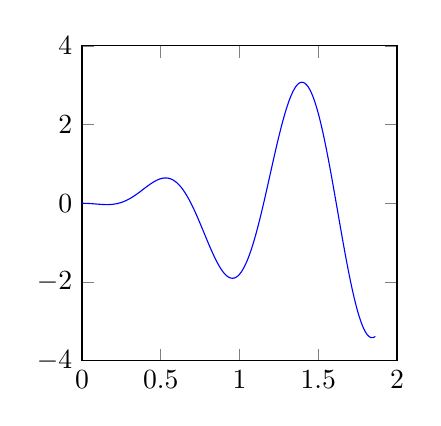
\begin{tikzpicture}

\begin{axis}[%
width=\figurewidth,
height=\figureheight,
scale only axis,
xmin=0,
xmax=2,
ymin=-4,
ymax=4
]
\addplot [color=blue,solid,forget plot]
  table[row sep=crcr]{%
0	0\\
0.00186206896551724	-9.81557918731428e-06\\
0.00372413793103448	-3.92485973868528e-05\\
0.00558620689655172	-8.82641320004888e-05\\
0.00744827586206897	-0.000156808154525201\\
0.00931034482758621	-0.000244807560818895\\
0.0111724137931034	-0.000352170209420864\\
0.0130344827586207	-0.000478784967915698\\
0.0148965517241379	-0.000624521767319481\\
0.0167586206896552	-0.000789231664470319\\
0.0186206896551724	-0.000972746912398953\\
0.0204827586206897	-0.00117488103865367\\
0.0223448275862069	-0.00139542893155333\\
0.0242068965517241	-0.0016341669343347\\
0.0260689655172414	-0.0018908529471638\\
0.0279310344827586	-0.00216522653697387\\
0.0297931034482759	-0.00245700905508991\\
0.0316551724137931	-0.00276590376260297\\
0.0335172413793103	-0.00309159596344666\\
0.0353793103448276	-0.00343375314513037\\
0.0372413793103448	-0.00379202512708536\\
0.0391034482758621	-0.00416604421656322\\
0.0409655172413793	-0.00455542537204366\\
0.0428275862068965	-0.0049597663740878\\
0.0446896551724138	-0.00537864800358338\\
0.046551724137931	-0.00581163422731614\\
0.0484137931034483	-0.0062582723908105\\
0.0502758620689655	-0.00671809341836777\\
0.0521379310344828	-0.00719061202023671\\
0.054	-0.00767532690684718\\
0.0558620689655172	-0.00817172101002975\\
0.0577241379310345	-0.0086792617111522\\
0.0595862068965517	-0.00919740107609054\\
0.061448275862069	-0.00972557609695757\\
0.0633103448275862	-0.0102632089405056\\
0.0651724137931034	-0.0108097072031222\\
0.0670344827586207	-0.0113644641723273\\
0.0688965517241379	-0.0119268590946905\\
0.0707586206896552	-0.0124962574500712\\
0.0726206896551724	-0.0130720112320935\\
0.0744827586206896	-0.0136534592347589\\
0.0763448275862069	-0.0142399273451013\\
0.0782068965517241	-0.0148307288417832\\
0.0800689655172414	-0.0154251646995372\\
0.0819310344827586	-0.0160225238993431\\
0.0837931034482759	-0.0166220837442425\\
0.0856551724137931	-0.0172231101806802\\
0.0875172413793103	-0.0178248581252654\\
0.0893793103448276	-0.0184265717968423\\
0.0912413793103448	-0.019027485053758\\
0.0931034482758621	-0.0196268217362131\\
0.0949655172413793	-0.0202237960135815\\
0.0968275862068965	-0.0208176127365785\\
0.0986896551724138	-0.0214074677941622\\
0.100551724137931	-0.0219925484750448\\
0.102413793103448	-0.0225720338336929\\
0.104275862068966	-0.0231450950606914\\
0.106137931034483	-0.0237108958573492\\
0.108	-0.024268592814415\\
0.109862068965517	-0.0248173357947798\\
0.111724137931034	-0.0253562683200327\\
0.113586206896552	-0.0258845279607415\\
0.115448275862069	-0.026401246730324\\
0.117310344827586	-0.0269055514823772\\
0.119172413793103	-0.0273965643113307\\
0.121034482758621	-0.0278734029562845\\
0.122896551724138	-0.0283351812078991\\
0.124758620689655	-0.0287810093181939\\
0.126620689655172	-0.0292099944131192\\
0.12848275862069	-0.0296212409077586\\
0.130344827586207	-0.03001385092402\\
0.132206896551724	-0.0303869247106758\\
0.134068965517241	-0.0307395610656031\\
0.135931034482759	-0.0310708577600861\\
0.137793103448276	-0.0313799119650312\\
0.139655172413793	-0.0316658206789497\\
0.14151724137931	-0.0319276811575626\\
0.143379310344828	-0.0321645913448785\\
0.145241379310345	-0.0323756503055976\\
0.147103448275862	-0.0325599586586926\\
0.148965517241379	-0.0327166190120181\\
0.150827586206897	-0.0328447363977961\\
0.152689655172414	-0.0329434187088317\\
0.154551724137931	-0.0330117771353033\\
0.156413793103448	-0.0330489266019807\\
0.158275862068966	-0.0330539862057153\\
0.160137931034483	-0.0330260796530559\\
0.162	-0.0329643356978319\\
0.163862068965517	-0.0328678885785568\\
0.165724137931034	-0.0327358784554969\\
0.167586206896552	-0.0325674518472536\\
0.169448275862069	-0.0323617620667063\\
0.171310344827586	-0.0321179696561639\\
0.173172413793103	-0.0318352428215708\\
0.175034482758621	-0.0315127578656171\\
0.176896551724138	-0.0311496996195988\\
0.178758620689655	-0.0307452618738761\\
0.180620689655172	-0.030298647806778\\
0.18248275862069	-0.029809070411802\\
0.184344827586207	-0.0292757529229552\\
0.186206896551724	-0.0286979292380885\\
0.188068965517241	-0.0280748443400706\\
0.189931034482759	-0.0274057547156529\\
0.191793103448276	-0.026689928771875\\
0.193655172413793	-0.0259266472498608\\
0.19551724137931	-0.0251152036358579\\
0.197379310344828	-0.0242549045693701\\
0.199241379310345	-0.0233450702482374\\
0.201103448275862	-0.0223850348305153\\
0.202965517241379	-0.0213741468330077\\
0.204827586206897	-0.0203117695263084\\
0.206689655172414	-0.0191972813262065\\
0.208551724137931	-0.0180300761813122\\
0.210413793103448	-0.0168095639567602\\
0.212275862068966	-0.015535170813849\\
0.214137931034483	-0.0142063395854758\\
0.216	-0.012822530147227\\
0.217862068965517	-0.0113832197839859\\
0.219724137931034	-0.0098879035519203\\
0.221586206896552	-0.0083360946357138\\
0.223448275862069	-0.00672732470090573\\
0.225310344827586	-0.00506114424120609\\
0.227172413793103	-0.00333712292065325\\
0.229034482758621	-0.00155484991048313\\
0.230896551724138	0.000286065779419632\\
0.232758620689655	0.00218599497461664\\
0.234620689655172	0.00414528801588362\\
0.23648275862069	0.00616427444477682\\
0.238344827586207	0.00824326269512078\\
0.240206896551724	0.0103825397905403\\
0.242068965517241	0.0125823710481567\\
0.243931034482759	0.0148429997885672\\
0.245793103448276	0.0171646470522243\\
0.247655172413793	0.0195475113223312\\
0.24951724137931	0.0219917682543657\\
0.251379310344828	0.0244975704123454\\
0.253241379310345	0.027065047011943\\
0.255103448275862	0.0296943036705609\\
0.256965517241379	0.0323854221644705\\
0.258827586206897	0.0351384601931194\\
0.260689655172414	0.0379534511507114\\
0.262551724137931	0.0408304039051558\\
0.264413793103448	0.0437693025844865\\
0.266275862068966	0.0467701063708472\\
0.268137931034483	0.0498327493021337\\
0.27	0.0529571400813884\\
0.271862068965517	0.0561431618940342\\
0.273724137931035	0.059390672233036\\
0.275586206896552	0.0626995027320748\\
0.277448275862069	0.0660694590068173\\
0.279310344827586	0.0695003205043603\\
0.281172413793103	0.0729918403609313\\
0.283034482758621	0.076543745267916\\
0.284896551724138	0.0801557353462911\\
0.286758620689655	0.0838274840295311\\
0.288620689655172	0.0875586379550571\\
0.29048275862069	0.0913488168642963\\
0.292344827586207	0.0951976135114118\\
0.294206896551724	0.0991045935807694\\
0.296068965517241	0.103069295613194\\
0.297931034482759	0.107091230941078\\
0.299793103448276	0.111169883632387\\
0.301655172413793	0.115304710443627\\
0.30351724137931	0.119495140781804\\
0.305379310344828	0.123740576675438\\
0.307241379310345	0.128040392754662\\
0.309103448275862	0.13239393624046\\
0.310965517241379	0.136800526943065\\
0.312827586206897	0.141259457269567\\
0.314689655172414	0.145769992240753\\
0.316551724137931	0.150331369517218\\
0.318413793103448	0.154942799434769\\
0.320275862068966	0.159603465049135\\
0.322137931034483	0.164312522190035\\
0.324	0.169069099524586\\
0.325862068965517	0.173872298630094\\
0.327724137931034	0.17872119407623\\
0.329586206896552	0.1836148335166\\
0.331448275862069	0.188552237789721\\
0.333310344827586	0.193532401029408\\
0.335172413793103	0.198554290784571\\
0.337034482758621	0.203616848148417\\
0.338896551724138	0.208718987897069\\
0.340758620689655	0.213859598637574\\
0.342620689655172	0.219037542965308\\
0.34448275862069	0.224251657630757\\
0.346344827586207	0.229500753715663\\
0.348206896551724	0.23478361681851\\
0.350068965517241	0.240099007249341\\
0.351931034482759	0.245445660233871\\
0.353793103448276	0.250822286126875\\
0.355655172413793	0.256227570634824\\
0.35751724137931	0.261660175047732\\
0.359379310344828	0.267118736480177\\
0.361241379310345	0.272601868121471\\
0.363103448275862	0.278108159494919\\
0.364965517241379	0.283636176726144\\
0.366827586206897	0.289184462820415\\
0.368689655172414	0.294751537948938\\
0.370551724137931	0.300335899744058\\
0.372413793103448	0.305936023603311\\
0.374275862068966	0.311550363002279\\
0.376137931034483	0.317177349816177\\
0.378	0.322815394650113\\
0.379862068965517	0.328462887177965\\
0.381724137931034	0.334118196489785\\
0.383586206896552	0.339779671447686\\
0.385448275862069	0.345445641050113\\
0.387310344827586	0.351114414804436\\
0.389172413793103	0.35678428310779\\
0.391034482758621	0.362453517636058\\
0.392896551724138	0.368120371740943\\
0.394758620689655	0.373783080855018\\
0.396620689655172	0.379439862904672\\
0.39848275862069	0.385088918730867\\
0.400344827586207	0.390728432517602\\
0.402206896551724	0.396356572227985\\
0.404068965517241	0.401971490047827\\
0.405931034482759	0.407571322836642\\
0.407793103448276	0.413154192585953\\
0.409655172413793	0.418718206884799\\
0.41151724137931	0.424261459392328\\
0.413379310344828	0.429782030317375\\
0.415241379310345	0.435277986904894\\
0.417103448275862	0.440747383929147\\
0.418965517241379	0.446188264193508\\
0.420827586206897	0.451598659036792\\
0.422689655172414	0.456976588845944\\
0.424551724137931	0.46232006357501\\
0.426413793103448	0.467627083270221\\
0.428275862068966	0.47289563860108\\
0.430137931034483	0.478123711397325\\
0.432	0.483309275191616\\
0.433862068965517	0.488450295767824\\
0.435724137931034	0.49354473171478\\
0.437586206896552	0.498590534985337\\
0.439448275862069	0.503585651460623\\
0.441310344827586	0.508528021519305\\
0.443172413793103	0.513415580611761\\
0.445034482758621	0.518246259838978\\
0.446896551724138	0.523017986536041\\
0.448758620689655	0.527728684860068\\
0.450620689655172	0.532376276382418\\
0.45248275862069	0.536958680685035\\
0.454344827586207	0.541473815960768\\
0.456206896551724	0.545919599617503\\
0.458068965517241	0.550293948885949\\
0.459931034482759	0.554594781430921\\
0.461793103448276	0.558820015965959\\
0.463655172413793	0.562967572871105\\
0.46551724137931	0.567035374813693\\
0.467379310344828	0.571021347371965\\
0.469241379310345	0.574923419661363\\
0.471103448275862	0.578739524963313\\
0.472965517241379	0.582467601356336\\
0.474827586206897	0.586105592349322\\
0.476689655172414	0.589651447516774\\
0.478551724137931	0.59310312313587\\
0.480413793103448	0.596458582825156\\
0.482275862068965	0.599715798184694\\
0.484137931034483	0.602872749437488\\
0.486	0.605927426072021\\
0.487862068965517	0.608877827485703\\
0.489724137931034	0.611721963629069\\
0.491586206896552	0.614457855650545\\
0.493448275862069	0.617083536541579\\
0.495310344827586	0.619597051781993\\
0.497172413793103	0.621996459985335\\
0.499034482758621	0.624279833544076\\
0.500896551724138	0.626445259274457\\
0.502758620689655	0.628490839060793\\
0.504620689655172	0.630414690499073\\
0.50648275862069	0.632214947539652\\
0.508344827586207	0.633889761128852\\
0.510206896551724	0.635437299849293\\
0.512068965517241	0.636855750558771\\
0.513931034482759	0.63814331902748\\
0.515793103448276	0.639298230573417\\
0.517655172413793	0.640318730695758\\
0.51951724137931	0.641203085706045\\
0.521379310344828	0.641949583356971\\
0.523241379310345	0.642556533468602\\
0.525103448275862	0.643022268551835\\
0.526965517241379	0.643345144428911\\
0.528827586206897	0.643523540850792\\
0.530689655172414	0.643555862111235\\
0.532551724137931	0.643440537657353\\
0.534413793103448	0.643176022696495\\
0.536275862068965	0.642760798799259\\
0.538137931034483	0.642193374498452\\
0.54	0.641472285883818\\
0.541862068965517	0.640596097192338\\
0.543724137931034	0.639563401393946\\
0.545586206896552	0.638372820772449\\
0.547448275862069	0.637023007501506\\
0.549310344827586	0.635512644215449\\
0.551172413793103	0.633840444574796\\
0.553034482758621	0.632005153826269\\
0.554896551724138	0.630005549357133\\
0.556758620689655	0.627840441243693\\
0.558620689655172	0.625508672793767\\
0.56048275862069	0.623009121082959\\
0.562344827586207	0.62034069748457\\
0.564206896551724	0.617502348192959\\
0.566068965517241	0.614493054740209\\
0.567931034482759	0.611311834505898\\
0.569793103448276	0.607957741219835\\
0.571655172413793	0.604429865457582\\
0.57351724137931	0.600727335128594\\
0.575379310344828	0.596849315956828\\
0.577241379310345	0.592795011953648\\
0.579103448275862	0.588563665882864\\
0.580965517241379	0.584154559717757\\
0.582827586206897	0.579567015089932\\
0.584689655172414	0.574800393729829\\
0.586551724137931	0.569854097898763\\
0.588413793103448	0.564727570812318\\
0.590275862068966	0.559420297054966\\
0.592137931034483	0.553931802985745\\
0.594	0.548261657134866\\
0.595862068965517	0.542409470591096\\
0.597724137931035	0.536374897379779\\
0.599586206896552	0.530157634831351\\
0.601448275862069	0.523757423940224\\
0.603310344827586	0.51717404971388\\
0.605172413793103	0.510407341512074\\
0.607034482758621	0.503457173375987\\
0.608896551724138	0.496323464347213\\
0.610758620689655	0.489006178776454\\
0.612620689655172	0.481505326621797\\
0.61448275862069	0.473820963736455\\
0.616344827586207	0.465953192145843\\
0.618206896551724	0.457902160313883\\
0.620068965517241	0.449668063398425\\
0.621931034482759	0.441251143495659\\
0.623793103448276	0.432651689873427\\
0.625655172413793	0.42387003919331\\
0.62751724137931	0.414906575721403\\
0.629379310344828	0.405761731527673\\
0.631241379310345	0.396435986673787\\
0.633103448275862	0.386929869389337\\
0.634965517241379	0.377243956236354\\
0.636827586206897	0.367378872262029\\
0.638689655172414	0.357335291139542\\
0.640551724137931	0.347113935296942\\
0.642413793103448	0.336715576033949\\
0.644275862068965	0.326141033626664\\
0.646137931034483	0.315391177420043\\
0.648	0.304466925908124\\
0.649862068965517	0.293369246801887\\
0.651724137931034	0.282099157084721\\
0.653586206896552	0.270657723055406\\
0.655448275862069	0.259046060358566\\
0.657310344827586	0.247265334002526\\
0.659172413793103	0.235316758364535\\
0.661034482758621	0.223201597183277\\
0.662896551724138	0.210921163538648\\
0.664758620689655	0.198476819818751\\
0.666620689655172	0.185869977674043\\
0.66848275862069	0.173102097958634\\
0.670344827586207	0.160174690658672\\
0.672206896551724	0.147089314807804\\
0.674068965517241	0.133847578389661\\
0.675931034482759	0.120451138227375\\
0.677793103448276	0.10690169986007\\
0.679655172413793	0.0932010174063413\\
0.68151724137931	0.079350893414683\\
0.683379310344828	0.0653531787008695\\
0.685241379310345	0.0512097721722685\\
0.687103448275862	0.0369226206390988\\
0.688965517241379	0.0224937186126111\\
0.690827586206897	0.00792510809020755\\
0.692689655172414	-0.00678112167249782\\
0.694551724137931	-0.021622834402677\\
0.696413793103448	-0.0365978470643081\\
0.698275862068966	-0.0517039301252449\\
0.700137931034483	-0.0669388078372642\\
0.702	-0.0823001585291173\\
0.703862068965517	-0.0977856149125212\\
0.705724137931035	-0.113392764401088\\
0.707586206896552	-0.129119149442143\\
0.709448275862069	-0.144962267861408\\
0.711310344827586	-0.160919573220491\\
0.713172413793103	-0.176988475187163\\
0.715034482758621	-0.193166339918363\\
0.716896551724138	-0.209450490455876\\
0.718758620689655	-0.225838207134646\\
0.720620689655172	-0.242326728003651\\
0.72248275862069	-0.258913249259291\\
0.724344827586207	-0.275594925691231\\
0.726206896551724	-0.292368871140608\\
0.728068965517241	-0.309232158970556\\
0.729931034482759	-0.326181822548973\\
0.731793103448276	-0.343214855743434\\
0.733655172413793	-0.360328213428194\\
0.73551724137931	-0.377518812003182\\
0.737379310344828	-0.394783529924907\\
0.739241379310345	-0.412119208249166\\
0.741103448275862	-0.429522651185513\\
0.742965517241379	-0.446990626663316\\
0.744827586206897	-0.464519866909372\\
0.746689655172414	-0.482107069036923\\
0.748551724137931	-0.499748895646021\\
0.750413793103448	-0.51744197543507\\
0.752275862068966	-0.535182903823492\\
0.754137931034483	-0.552968243585347\\
0.756	-0.570794525493843\\
0.757862068965517	-0.588658248976563\\
0.759724137931034	-0.606555882781318\\
0.761586206896552	-0.624483865652484\\
0.763448275862069	-0.64243860701768\\
0.765310344827586	-0.660416487684699\\
0.767172413793103	-0.678413860548483\\
0.769034482758621	-0.696427051308071\\
0.770896551724138	-0.714452359193322\\
0.772758620689655	-0.732486057701319\\
0.774620689655172	-0.750524395342251\\
0.77648275862069	-0.768563596394667\\
0.778344827586207	-0.786599861669912\\
0.780206896551724	-0.80462936928562\\
0.782068965517241	-0.822648275448076\\
0.783931034482759	-0.840652715243304\\
0.785793103448276	-0.858638803436699\\
0.787655172413793	-0.876602635281054\\
0.78951724137931	-0.894540287332788\\
0.791379310344828	-0.912447818276233\\
0.793241379310345	-0.930321269755765\\
0.795103448275862	-0.948156667215639\\
0.796965517241379	-0.96595002074732\\
0.798827586206897	-0.983697325944142\\
0.800689655172414	-1.00139456476311\\
0.802551724137931	-1.01903770639363\\
0.804413793103448	-1.03662270813303\\
0.806275862068966	-1.05414551626864\\
0.808137931034483	-1.07160206696622\\
0.81	-1.08898828716459\\
0.811862068965517	-1.10630009547625\\
0.813724137931034	-1.12353340309376\\
0.815586206896552	-1.14068411470167\\
0.817448275862069	-1.15774812939389\\
0.819310344827586	-1.17472134159613\\
0.821172413793103	-1.19159964199341\\
0.823034482758621	-1.2083789184622\\
0.824896551724138	-1.22505505700717\\
0.826758620689655	-1.24162394270226\\
0.828620689655172	-1.25808146063576\\
0.83048275862069	-1.27442349685944\\
0.832344827586207	-1.29064593934118\\
0.834206896551724	-1.30674467892118\\
0.836068965517241	-1.32271561027131\\
0.837931034482759	-1.33855463285751\\
0.839793103448276	-1.35425765190498\\
0.841655172413793	-1.36982057936584\\
0.84351724137931	-1.38523933488926\\
0.845379310344828	-1.40050984679354\\
0.847241379310345	-1.41562805304017\\
0.849103448275862	-1.43058990220948\\
0.850965517241379	-1.4453913544777\\
0.852827586206897	-1.46002838259521\\
0.854689655172414	-1.47449697286571\\
0.856551724137931	-1.48879312612616\\
0.858413793103448	-1.50291285872708\\
0.860275862068966	-1.51685220351325\\
0.862137931034483	-1.53060721080421\\
0.864	-1.54417394937472\\
0.865862068965517	-1.55754850743462\\
0.867724137931035	-1.57072699360804\\
0.869586206896552	-1.58370553791162\\
0.871448275862069	-1.59648029273158\\
0.873310344827586	-1.60904743379932\\
0.875172413793103	-1.62140316116541\\
0.877034482758621	-1.63354370017161\\
0.878896551724138	-1.64546530242077\\
0.880758620689655	-1.65716424674438\\
0.882620689655172	-1.6686368401674\\
0.88448275862069	-1.67987941887032\\
0.886344827586207	-1.69088834914804\\
0.888206896551724	-1.70166002836545\\
0.890068965517241	-1.7121908859094\\
0.891931034482759	-1.7224773841368\\
0.893793103448276	-1.73251601931877\\
0.895655172413793	-1.74230332258036\\
0.89751724137931	-1.75183586083578\\
0.899379310344828	-1.76111023771883\\
0.901241379310345	-1.77012309450837\\
0.903103448275862	-1.77887111104844\\
0.904965517241379	-1.78735100666293\\
0.906827586206897	-1.79555954106455\\
0.908689655172414	-1.80349351525777\\
0.910551724137931	-1.81114977243564\\
0.912413793103448	-1.81852519887012\\
0.914275862068965	-1.82561672479576\\
0.916137931034483	-1.83242132528648\\
0.918	-1.83893602112529\\
0.919862068965517	-1.84515787966654\\
0.921724137931034	-1.85108401569071\\
0.923586206896552	-1.85671159225129\\
0.925448275862069	-1.86203782151373\\
0.927310344827586	-1.86705996558604\\
0.929172413793103	-1.87177533734095\\
0.931034482758621	-1.87618130122941\\
0.932896551724138	-1.88027527408512\\
0.934758620689655	-1.88405472591992\\
0.936620689655172	-1.88751718070989\\
0.93848275862069	-1.89066021717181\\
0.940344827586207	-1.89348146952989\\
0.942206896551724	-1.8959786282725\\
0.944068965517241	-1.89814944089869\\
0.945931034482759	-1.89999171265432\\
0.947793103448276	-1.90150330725756\\
0.949655172413793	-1.90268214761362\\
0.95151724137931	-1.90352621651842\\
0.953379310344827	-1.90403355735105\\
0.955241379310345	-1.90420227475488\\
0.957103448275862	-1.90403053530698\\
0.958965517241379	-1.90351656817583\\
0.960827586206896	-1.90265866576697\\
0.962689655172414	-1.90145518435654\\
0.964551724137931	-1.89990454471246\\
0.966413793103448	-1.89800523270297\\
0.968275862068965	-1.89575579989265\\
0.970137931034483	-1.89315486412533\\
0.972	-1.89020111009409\\
0.973862068965517	-1.88689328989794\\
0.975724137931034	-1.88323022358511\\
0.977586206896552	-1.87921079968277\\
0.979448275862069	-1.87483397571303\\
0.981310344827586	-1.87009877869496\\
0.983172413793103	-1.86500430563268\\
0.985034482758621	-1.85954972398914\\
0.986896551724138	-1.85373427214557\\
0.988758620689655	-1.8475572598464\\
0.990620689655172	-1.84101806862959\\
0.99248275862069	-1.83411615224208\\
0.994344827586207	-1.82685103704035\\
0.996206896551724	-1.81922232237589\\
0.998068965517241	-1.81122968096549\\
0.999931034482759	-1.80287285924615\\
1.00179310344828	-1.79415167771457\\
1.00365517241379	-1.78506603125105\\
1.00551724137931	-1.77561588942767\\
1.00737931034483	-1.7658012968007\\
1.00924137931034	-1.75562237318698\\
1.01110344827586	-1.74507931392443\\
1.01296551724138	-1.73417239011622\\
1.0148275862069	-1.72290194885885\\
1.01668965517241	-1.71126841345382\\
1.01855172413793	-1.69927228360288\\
1.02041379310345	-1.68691413558676\\
1.02227586206897	-1.67419462242723\\
1.02413793103448	-1.66111447403259\\
1.026	-1.64767449732623\\
1.02786206896552	-1.63387557635847\\
1.02972413793103	-1.6197186724014\\
1.03158620689655	-1.60520482402676\\
1.03344827586207	-1.59033514716674\\
1.03531034482759	-1.57511083515772\\
1.0371724137931	-1.55953315876676\\
1.03903448275862	-1.54360346620095\\
1.04089655172414	-1.52732318309944\\
1.04275862068966	-1.51069381250813\\
1.04462068965517	-1.49371693483709\\
1.04648275862069	-1.4763942078005\\
1.04834482758621	-1.4587273663392\\
1.05020689655172	-1.44071822252582\\
1.05206896551724	-1.42236866545236\\
1.05393103448276	-1.40368066110033\\
1.05579310344828	-1.38465625219338\\
1.05765517241379	-1.36529755803233\\
1.05951724137931	-1.34560677431276\\
1.06137931034483	-1.32558617292503\\
1.06324137931034	-1.30523810173669\\
1.06510344827586	-1.2845649843575\\
1.06696551724138	-1.26356931988678\\
1.0688275862069	-1.24225368264335\\
1.07068965517241	-1.22062072187791\\
1.07255172413793	-1.198673161468\\
1.07441379310345	-1.17641379959545\\
1.07627586206897	-1.15384550840647\\
1.07813793103448	-1.1309712336543\\
1.08	-1.10779399432453\\
1.08186206896552	-1.08431688224316\\
1.08372413793103	-1.06054306166728\\
1.08558620689655	-1.03647576885867\\
1.08744827586207	-1.01211831164013\\
1.08931034482759	-0.987474068934819\\
1.0911724137931	-0.962546490288424\\
1.09303448275862	-0.937339095374474\\
1.09489655172414	-0.911855473482685\\
1.09675862068966	-0.886099282990505\\
1.09862068965517	-0.860074250817898\\
1.10048275862069	-0.833784171865461\\
1.10234482758621	-0.807232908435964\\
1.10420689655172	-0.78042438963941\\
1.10606896551724	-0.753362610781681\\
1.10793103448276	-0.726051632736905\\
1.10979310344828	-0.698495581303635\\
1.11165517241379	-0.670698646544895\\
1.11351724137931	-0.642665082112342\\
1.11537931034483	-0.614399204554451\\
1.11724137931034	-0.585905392609072\\
1.11910344827586	-0.55718808648028\\
1.12096551724138	-0.528251787099785\\
1.1228275862069	-0.499101055372936\\
1.12468965517241	-0.469740511409543\\
1.12655172413793	-0.440174833739573\\
1.12841379310345	-0.410408758513911\\
1.13027586206897	-0.38044707869031\\
1.13213793103448	-0.350294643204681\\
1.134	-0.319956356127899\\
1.13586206896552	-0.289437175808249\\
1.13772413793103	-0.258742113999691\\
1.13958620689655	-0.227876234976094\\
1.14144827586207	-0.196844654631626\\
1.14331034482759	-0.165652539567445\\
1.1451724137931	-0.134305106164915\\
1.14703448275862	-0.102807619645439\\
1.14889655172414	-0.0711653931171906\\
1.15075862068965	-0.0393837866088264\\
1.15262068965517	-0.00746820609047376\\
1.15448275862069	0.0245758975179002\\
1.15634482758621	0.0567430293505014\\
1.15820689655172	0.0890276516119292\\
1.16006896551724	0.121424184605382\\
1.16193103448276	0.153927007772639\\
1.16379310344828	0.18653046074566\\
1.16565517241379	0.219228844409508\\
1.16751724137931	0.252016421976482\\
1.16937931034483	0.284887420071166\\
1.17124137931034	0.317836029826191\\
1.17310344827586	0.350856407988532\\
1.17496551724138	0.383942678036045\\
1.1768275862069	0.417088931304075\\
1.17868965517241	0.450289228121873\\
1.18055172413793	0.483537598958629\\
1.18241379310345	0.516828045578793\\
1.18427586206897	0.550154542206551\\
1.18613793103448	0.583511036699169\\
1.188	0.61689145172896\\
1.18986206896552	0.650289685973619\\
1.19172413793103	0.683699615314713\\
1.19358620689655	0.717115094044015\\
1.19544827586207	0.75052995607753\\
1.19731034482759	0.783938016176824\\
1.1991724137931	0.817333071177532\\
1.20103448275862	0.85070890122469\\
1.20289655172414	0.88405927101465\\
1.20475862068966	0.917377931043391\\
1.20662068965517	0.950658618860812\\
1.20848275862069	0.98389506033091\\
1.21034482758621	1.01708097089743\\
1.21220689655172	1.05021005685482\\
1.21406896551724	1.08327601662411\\
1.21593103448276	1.11627254203361\\
1.21779310344828	1.14919331960395\\
1.21965517241379	1.18203203183734\\
1.22151724137931	1.21478235851071\\
1.22337931034483	1.2474379779724\\
1.22524137931034	1.27999256844227\\
1.22710344827586	1.31243980931476\\
1.22896551724138	1.34477338246478\\
1.2308275862069	1.37698697355603\\
1.23268965517241	1.40907427335151\\
1.23455172413793	1.44102897902596\\
1.23641379310345	1.47284479547986\\
1.23827586206897	1.50451543665486\\
1.24013793103448	1.53603462685009\\
1.242	1.56739610203938\\
1.24386206896552	1.59859361118881\\
1.24572413793103	1.6296209175745\\
1.24758620689655	1.66047180010024\\
1.24944827586207	1.69114005461471\\
1.25131034482759	1.72161949522796\\
1.2531724137931	1.75190395562694\\
1.25503448275862	1.78198729038971\\
1.25689655172414	1.81186337629802\\
1.25875862068966	1.84152611364805\\
1.26062068965517	1.87096942755897\\
1.26248275862069	1.90018726927899\\
1.26434482758621	1.92917361748869\\
1.26620689655172	1.95792247960128\\
1.26806896551724	1.98642789305949\\
1.26993103448276	2.01468392662882\\
1.27179310344828	2.04268468168686\\
1.27365517241379	2.0704242935084\\
1.27551724137931	2.09789693254601\\
1.27737931034483	2.12509680570574\\
1.27924137931034	2.15201815761788\\
1.28110344827586	2.17865527190213\\
1.28296551724138	2.20500247242724\\
1.2848275862069	2.23105412456465\\
1.28668965517241	2.25680463643582\\
1.28855172413793	2.28224846015307\\
1.29041379310345	2.3073800930536\\
1.29227586206897	2.33219407892636\\
1.29413793103448	2.35668500923155\\
1.296	2.3808475243125\\
1.29786206896552	2.40467631459945\\
1.29972413793103	2.42816612180528\\
1.30158620689655	2.45131174011258\\
1.30344827586207	2.47410801735204\\
1.30531034482759	2.49654985617168\\
1.3071724137931	2.51863221519687\\
1.30903448275862	2.54035011018061\\
1.31089655172414	2.56169861514405\\
1.31275862068966	2.5826728635068\\
1.31462068965517	2.60326804920689\\
1.31648275862069	2.62347942780997\\
1.31834482758621	2.64330231760768\\
1.32020689655172	2.6627321007048\\
1.32206896551724	2.68176422409489\\
1.32393103448276	2.70039420072433\\
1.32579310344828	2.71861761054428\\
1.32765517241379	2.73643010155058\\
1.32951724137931	2.7538273908111\\
1.33137931034483	2.77080526548037\\
1.33324137931034	2.78735958380135\\
1.33510344827586	2.80348627609396\\
1.33696551724138	2.81918134573023\\
1.3388275862069	2.83444087009571\\
1.34068965517241	2.84926100153711\\
1.34255172413793	2.86363796829571\\
1.34441379310345	2.87756807542654\\
1.34627586206897	2.89104770570286\\
1.34813793103448	2.90407332050594\\
1.35	2.91664146069982\\
1.35186206896552	2.92874874749085\\
1.35372413793103	2.94039188327174\\
1.35558620689655	2.95156765245004\\
1.35744827586207	2.96227292226073\\
1.35931034482759	2.97250464356278\\
1.3611724137931	2.98225985161945\\
1.36303448275862	2.99153566686216\\
1.36489655172414	3.00032929563768\\
1.36675862068966	3.00863803093857\\
1.36862068965517	3.01645925311657\\
1.37048275862069	3.02379043057877\\
1.37234482758621	3.03062912046646\\
1.37420689655172	3.03697296931646\\
1.37606896551724	3.04281971370463\\
1.37793103448276	3.04816718087165\\
1.37979310344828	3.05301328933062\\
1.38165517241379	3.05735604945658\\
1.38351724137931	3.06119356405757\\
1.38537931034483	3.06452402892729\\
1.38724137931034	3.06734573337898\\
1.38910344827586	3.06965706076065\\
1.39096551724138	3.07145648895127\\
1.3928275862069	3.0727425908379\\
1.39468965517241	3.07351403477369\\
1.39655172413793	3.07376958501649\\
1.39841379310345	3.07350810214801\\
1.40027586206897	3.07272854347342\\
1.40213793103448	3.07142996340134\\
1.404	3.0696115138039\\
1.40586206896552	3.06727244435701\\
1.40772413793103	3.06441210286063\\
1.40958620689655	3.06102993553884\\
1.41144827586207	3.05712548731988\\
1.41331034482759	3.05269840209576\\
1.4151724137931	3.04774842296163\\
1.41703448275862	3.04227539243464\\
1.41889655172414	3.0362792526523\\
1.42075862068966	3.0297600455503\\
1.42262068965517	3.0227179130196\\
1.42448275862069	3.01515309704288\\
1.42634482758621	3.00706593981022\\
1.42820689655172	2.99845688381388\\
1.43006896551724	2.98932647192233\\
1.43193103448276	2.9796753474333\\
1.43379310344828	2.96950425410585\\
1.43565517241379	2.95881403617157\\
1.43751724137931	2.94760563832466\\
1.43937931034483	2.93588010569106\\
1.44124137931034	2.92363858377641\\
1.44310344827586	2.91088231839311\\
1.44496551724138	2.89761265556616\\
1.4468275862069	2.88383104141794\\
1.44868965517241	2.86953902203197\\
1.45055172413793	2.85473824329555\\
1.45241379310345	2.83943045072127\\
1.45427586206897	2.82361748924756\\
1.45613793103448	2.80730130301815\\
1.458	2.79048393514046\\
1.45986206896552	2.77316752742312\\
1.46172413793103	2.75535432009242\\
1.46358620689655	2.73704665148785\\
1.46544827586207	2.71824695773687\\
1.46731034482759	2.69895777240865\\
1.4691724137931	2.67918172614723\\
1.47103448275862	2.65892154628378\\
1.47289655172414	2.63818005642833\\
1.47475862068966	2.61696017604078\\
1.47662068965517	2.59526491998148\\
1.47848275862069	2.57309739804124\\
1.48034482758621	2.55046081445104\\
1.48220689655172	2.52735846737145\\
1.48406896551724	2.50379374836176\\
1.48593103448276	2.47977014182907\\
1.48779310344828	2.4552912244573\\
1.48965517241379	2.43036066461634\\
1.49151724137931	2.40498222175134\\
1.49337931034483	2.37915974575235\\
1.49524137931034	2.35289717630426\\
1.49710344827586	2.32619854221745\\
1.49896551724138	2.29906796073892\\
1.5008275862069	2.27150963684433\\
1.50268965517241	2.24352786251089\\
1.50455172413793	2.21512701597134\\
1.50641379310345	2.18631156094911\\
1.50827586206897	2.15708604587483\\
1.51013793103448	2.12745510308432\\
1.512	2.09742344799826\\
1.51386206896552	2.06699587828364\\
1.51572413793103	2.03617727299715\\
1.51758620689655	2.0049725917108\\
1.51944827586207	1.97338687361971\\
1.52131034482759	1.94142523663254\\
1.5231724137931	1.90909287644444\\
1.52503448275862	1.87639506559295\\
1.52689655172414	1.84333715249682\\
1.52875862068966	1.80992456047818\\
1.53062068965517	1.77616278676804\\
1.53248275862069	1.74205740149544\\
1.53434482758621	1.70761404666037\\
1.53620689655172	1.67283843509083\\
1.53806896551724	1.63773634938397\\
1.53993103448276	1.60231364083181\\
1.54179310344828	1.56657622833155\\
1.54365517241379	1.5305300972808\\
1.54551724137931	1.49418129845791\\
1.54737931034483	1.45753594688764\\
1.54924137931034	1.42060022069238\\
1.55110344827586	1.38338035992923\\
1.55296551724138	1.34588266541308\\
1.5548275862069	1.30811349752595\\
1.55668965517241	1.27007927501297\\
1.55855172413793	1.23178647376492\\
1.56041379310345	1.1932416255881\\
1.56227586206897	1.15445131696118\\
1.56413793103448	1.11542218777982\\
1.566	1.0761609300889\\
1.56786206896552	1.03667428680298\\
1.56972413793103	0.996969050414972\\
1.57158620689655	0.957052061693447\\
1.57344827586207	0.916930208368785\\
1.57531034482759	0.876610423808494\\
1.5771724137931	0.836099685681924\\
1.57903448275862	0.795405014614693\\
1.58089655172414	0.754533472833041\\
1.58275862068966	0.713492162798518\\
1.58462068965517	0.672288225833134\\
1.58648275862069	0.630928840735399\\
1.58834482758621	0.589421222387485\\
1.59020689655172	0.547772620353747\\
1.59206896551724	0.505990317471045\\
1.59393103448276	0.464081628430972\\
1.59579310344828	0.422053898354493\\
1.59765517241379	0.379914501359069\\
1.59951724137931	0.337670839118835\\
1.60137931034483	0.295330339417868\\
1.60324137931034	0.252900454697023\\
1.60510344827586	0.210388660594604\\
1.60696551724138	0.167802454481152\\
1.6088275862069	0.125149353988706\\
1.61068965517241	0.0824368955347899\\
1.61255172413793	0.0396726328414738\\
1.61441379310345	-0.00313586455014921\\
1.61627586206897	-0.0459810127698149\\
1.61813793103448	-0.0888552151118905\\
1.62	-0.131750863532865\\
1.62186206896552	-0.174660340152219\\
1.62372413793103	-0.217576018756199\\
1.62558620689655	-0.260490266304447\\
1.62744827586207	-0.303395444438885\\
1.62931034482759	-0.346283910994752\\
1.6311724137931	-0.389148021513328\\
1.63303448275862	-0.431980130756066\\
1.63489655172414	-0.47477259421984\\
1.63675862068966	-0.517517769652992\\
1.63862068965517	-0.5602080185717\\
1.64048275862069	-0.602835707776611\\
1.64234482758621	-0.645393210869144\\
1.64420689655172	-0.68787290976735\\
1.64606896551724	-0.730267196220853\\
1.64793103448276	-0.772568473324615\\
1.64979310344828	-0.814769157031215\\
1.65165517241379	-0.856861677661293\\
1.65351724137931	-0.898838481411805\\
1.65537931034483	-0.940692031861823\\
1.65724137931034	-0.982414811475503\\
1.65910344827586	-1.02399932310194\\
1.66096551724138	-1.06543809147161\\
1.6628275862069	-1.1067236646889\\
1.66468965517241	-1.14784861572074\\
1.66655172413793	-1.18880554388062\\
1.66841379310345	-1.22958707630801\\
1.67027586206897	-1.27018586944265\\
1.67213793103448	-1.31059461049349\\
1.674	-1.35080601890192\\
1.67586206896552	-1.39081284779905\\
1.67772413793103	-1.43060788545653\\
1.67958620689655	-1.47018395673094\\
1.68144827586207	-1.50953392450099\\
1.68331034482759	-1.54865069109771\\
1.6851724137931	-1.58752719972684\\
1.68703448275862	-1.62615643588352\\
1.68889655172414	-1.66453142875869\\
1.69075862068966	-1.70264525263706\\
1.69262068965517	-1.74049102828627\\
1.69448275862069	-1.77806192433695\\
1.69634482758621	-1.81535115865342\\
1.69820689655172	-1.85235199969466\\
1.70006896551724	-1.88905776786537\\
1.70193103448276	-1.92546183685665\\
1.70379310344828	-1.96155763497626\\
1.70565517241379	-1.99733864646787\\
1.70751724137931	-2.03279841281928\\
1.70937931034483	-2.06793053405921\\
1.71124137931034	-2.10272867004232\\
1.71310344827586	-2.13718654172233\\
1.71496551724138	-2.17129793241282\\
1.7168275862069	-2.20505668903552\\
1.71868965517241	-2.23845672335581\\
1.72055172413793	-2.27149201320515\\
1.72241379310345	-2.30415660369013\\
1.72427586206897	-2.33644460838801\\
1.72613793103448	-2.36835021052827\\
1.728	-2.3998676641602\\
1.72986206896552	-2.43099129530599\\
1.73172413793103	-2.46171550309931\\
1.73358620689655	-2.49203476090891\\
1.73544827586207	-2.52194361744722\\
1.73731034482759	-2.55143669786355\\
1.7391724137931	-2.58050870482167\\
1.74103448275862	-2.60915441956166\\
1.74289655172414	-2.63736870294562\\
1.74475862068966	-2.66514649648711\\
1.74662068965517	-2.69248282336419\\
1.74848275862069	-2.71937278941559\\
1.75034482758621	-2.74581158412003\\
1.75220689655172	-2.77179448155841\\
1.75406896551724	-2.79731684135852\\
1.75593103448276	-2.82237410962239\\
1.75779310344828	-2.84696181983562\\
1.75965517241379	-2.87107559375896\\
1.76151724137931	-2.89471114230165\\
1.76337931034483	-2.91786426637638\\
1.76524137931034	-2.94053085773578\\
1.76710344827586	-2.96270689979017\\
1.76896551724138	-2.98438846840641\\
1.7708275862069	-3.00557173268775\\
1.77268965517241	-3.02625295573431\\
1.77455172413793	-3.04642849538433\\
1.77641379310345	-3.06609480493576\\
1.77827586206897	-3.08524843384816\\
1.78013793103448	-3.10388602842476\\
1.782	-3.12200433247443\\
1.78386206896552	-3.13960018795364\\
1.78572413793103	-3.15667053558795\\
1.78758620689655	-3.17321241547324\\
1.78944827586207	-3.18922296765625\\
1.79131034482759	-3.2046994326945\\
1.7931724137931	-3.21963915219543\\
1.79503448275862	-3.23403956933457\\
1.79689655172414	-3.2478982293527\\
1.79875862068966	-3.26121278003185\\
1.80062068965517	-3.27398097215016\\
1.80248275862069	-3.28620065991525\\
1.80434482758621	-3.29786980137628\\
1.80620689655172	-3.30898645881447\\
1.80806896551724	-3.31954879911196\\
1.80993103448276	-3.32955509409908\\
1.81179310344828	-3.33900372087978\\
1.81365517241379	-3.34789316213535\\
1.81551724137931	-3.35622200640613\\
1.81737931034483	-3.36398894835135\\
1.81924137931034	-3.371192788987\\
1.82110344827586	-3.37783243590154\\
1.82296551724138	-3.38390690344966\\
1.8248275862069	-3.38941531292378\\
1.82668965517241	-3.39435689270347\\
1.82855172413793	-3.39873097838265\\
1.83041379310345	-3.40253701287454\\
1.83227586206897	-3.40577454649439\\
1.83413793103448	-3.40844323701999\\
1.836	-3.41054284972983\\
1.83786206896552	-3.41207325741903\\
1.83972413793103	-3.41303444039307\\
1.84158620689655	-3.41342648643908\\
1.84344827586207	-3.41324959077505\\
1.84531034482759	-3.4125040559767\\
1.8471724137931	-3.41119029188209\\
1.84903448275862	-3.40930881547414\\
1.85089655172414	-3.4068602507409\\
1.85275862068966	-3.40384532851367\\
1.85462068965517	-3.40026488628306\\
1.85648275862069	-3.39611986799301\\
1.85834482758621	-3.39141132381271\\
1.86020689655172	-3.38614040988669\\
1.86206896551724	-3.3803083880629\\
};
\end{axis}
\end{tikzpicture}% 
\caption{Time history of dynamic amplification factor in mid-span of the beam. Parameters:$EJ=2.43e10Nm^2$,$L=54m$,$\mu=6000kg/m$,$c=29.26m/s$} 
\label{fig:EJ24300000000L54mu6000c29daf.tikz} 
\end{figure}

By observing Figure.\ref{fig:hilalplot} and Figure.\ref{fig:EJ24300000000L54mu6000c29daf.tikz} it can be concluded that results are the same on y-axis. The difference of x-axis is because in Figure.\ref{fig:hilalplot} time axis is scaled to 1 but in Figure.\ref{fig:EJ24300000000L54mu6000c29daf.tikz} time is not scaled. Then it can be further concluded that Eq.\ref{eq:v(x,t)simpleharmonic} and expression for $\omega_b$ are both correct.

\section{Parameter calculation}
The parameters needed for solving the explicit solution(Eq.\ref{eq:v(x,t)simpleharmonic}) are:

\begin{table}[h!]
	\centering
	\begin{tabular}{cc}
		\hline
		$l$ & Length of the beam \\ 
		$\zeta$ & Damping ratio \\
		$Q$ & Amplitude of the load \\
		$EJ$ & Lateral stiffness of the beam \\
		$\mu$ & Mass per unit length \\
		$c$ & Speed of train \\
		\hline
	\end{tabular}
\end{table}
	

Despite parameter $Q$, other parameters are the fundamental attributes of bridge and vehicle which do not need further derivation. Thus this section aims to derive the expression for $Q$.

The expression of $Q$ will be determined in following sequence:

Firstly a \emph{hypothesis expression} for amplitude $Q$ will be made depend on a \emph{peak lateral force model}. Then the hypothesis amplitude, together with the explicit solution embedding it, will be validated by confirming if the explicit solution is able to reproduce similar results with numerical vehicle-bridge resonance simulations.\footnote{Lateral resonance research\citep[Figure.C1,C2,...,C30]{d181dt329} provides input and output data of these simulations}.

Paragraphs in this section are arranged accordingly to above sequence. They are written in following layout:

\begin{enumerate}
	\item Peak lateral model
	\item Hypothesis expression for $Q$
	\item Validation of the explicit solution
\end{enumerate}

\subsection{Peak lateral force model}\label{sec:peaklateralforcemodel}

The peak lateral force model is obtained by statistically fitting the peak force results of different train speeds provided by UIC research\citep{d181dt329}. The model is expected to describe the relationship between peak lateral force and train speed. 

The peak lateral force of different train types under different train speeds are presented in Table.\ref{tab:peaklateralforce}. Two figures(bold numbers) are modified\footnote{
	The original values are 160 and 250 respectively. Output data in the table should have been filtered by standard deviation filter. The table data does not represent true maximum lateral force but a value greater than 99.5\% of all force values. However, it is obvious that output data of 160kN was not filtered. It is the greatest value among all raw output data of freight train running at 100 km/h. It is not possible to calculate the explicit standard value because raw data are presented in the form of chart image. The modified value of 80kN is obtained by approximate observation. As a result, the total lateral force is modified to 170kN.} from original table.
The data in the table will be used to create the speed-based expression for peak lateral force model. 

\begin{table}[h!]
    \centering
    \caption{Peak Lateral Track Force Over All Track Qualities. Extracted From \citet[Tab. B1]{d181dt329}}
    \begin{tabular}{cccc}

        \hline
         & \multicolumn{3}{c}{Peak lateral force(kN)} \\
        Train type and speed & Locomotive & Coach/Wagon & Total \\ 
        \hline
        Freight 60 km/h & 50 & 60 & 110\\
        Freight 100 km/h & 90 & \textbf{\textit{80}}& \textbf{\textit{170}}\\
        Freight 120 km/h & 75 & 110 & 185 \\
        Passenger 200 km/h & 140 & 50 & 190 \\
        High Speed 350 km/h & 125 & 125 & 250 \\
        Passenger 200 km/h(worn) & 190 & 80 & 270 \\
        High Speed 350 km/h & 330 & 225 & 555 \\
        \hline
    \end{tabular}
    \label{tab:peaklateralforce}
\end{table}

The model is created by fitting the data in Table.\ref{tab:peaklateralforce} to a function. The function should be able to satisfy following characteristics:

\begin{enumerate}
	\item 0kN lateral force when speed is 0km/h
	\item Simply increasing in value but generally decreasing in increment\footnote{It can be observed from Table.\ref{tab:peaklateralforce}  that the relationship between lateral force and speed is not linear. The fact that force increment decreases as speed increases can also be observed.}
\end{enumerate}

Finally function form $F=a*v^b$ is selected because its satisfying characteristics. The first regression is conducted according to freight train data because it possesses the most sets of data. R language was used to perform regression process. 

The fitting result is presented in Formula.\ref{for:regressionfreight}. It is in good likelihood with original data. Achieved convergence tolerance is $2.868e-06$.  See Appendix.\ref{sec:Rregression} for code.

\begin{equation}
\label{for:regressionfreight}
F_{lf} = 5.2064\cdot v^{0.7495}
\end{equation}

Since 1 set of data is available for passenger train, Formula.\ref{for:regressionfreight} is scaled by a constant factor to create regression for passenger trains. Please note that this regression can not be verified because lack of data. However, since freight train has a greater lateral force then passenger train, it is conservative to adopt lateral force of freight train when calculating consequences related to passenger trains. It is still reasonable to adopt this regression since passenger trains are just simply less stiff than freight trains. 

The scale factor $k_{pf}$ is obtained by comparing force value yielded by Formula.\ref{for:regressionfreight} at 200km/h and original passenger train force(190kN) data at 200km/h.

$$k_{pf} = \frac{190}{a_{lf}\cdot 200^{b_{lf}}}$$
$$a_{lp} = a_{lf}\cdot k_{pf}$$
merge above two equations, yield
$$a_{lp} = \frac{190}{200^{b_{lf}}} = \frac{190}{200^{0.7495}} \approx 3.58$$

and 

$$F_{lp} = a_{lp}\cdot v^{0.7495}$$

thus

\begin{equation}\label{for:regressionpassenger}
F_{lp} = 3.58\cdot v^{0.7495}
\end{equation}

Lateral force for high speed train were obtained in same manner. The scale factor $k_{hf}$ is obtained by comparing force value yielded by Formula.\ref{for:regressionfreight} at 350km/h and original high speed train force(250kN) data at 350km/h.

$$k_{hf} = \frac{250}{a_{lf}\cdot 350^{b_{lf}}}$$
$$a_{lh} = a_{lf}\cdot k_{hf}$$
merge above two equations, yield
$$a_{lh} = \frac{250}{350^{b_{lf}}} = \frac{250}{350^{0.7495}} \approx 3.10$$

and 

$$F_{lh} = a_{lh}\cdot v^{0.7495}$$
thus

\begin{equation}\label{for:regressionhighspeed}
F_{lh} = 3.10\cdot v^{0.7495}
\end{equation}


\begin{figure}[h!]
    \centering
    \begin{tikzpicture}
    \begin{axis}[
    % title = {Peak lateral track forces over all track qualities(worn profile scenario neglected)},
    width = 0.9\textwidth,
    xlabel={$v(km/s)$},
    ylabel={$F(kN)$},
    ymin = 0, xmin = 0, xmax = 350,
    grid = both,
    ytick = {50,100,...,250},
    xtick = {60,100,120,200,350},
    legend style={
    at={(0,0)},
    anchor=north west,at={(axis description cs:0.45,0.43)}}] 
    ]
    \addplot[name path = C,mark=*, green] coordinates {(200,190) (350,250)};
    \addplot[blue,name path = B,mark=*] coordinates {(120,185) (200,190)};
    \addplot[red,name path = A,mark=*] coordinates {(0,0) (60,110) (100,170) (120,185)};
    \addplot[red,name path = D, domain = 0:120, dashed]{5.2064*x^0.7498};
    \addplot[blue,name path = E, domain = 0:200, dashed]{3.58*x^0.7498};
    \addplot[name path = F, domain = 0:350, dashed, green]{3.1*x^0.7498};
    \addplot[domain = 0:350] {100};
    \legend{high speed train, passenger train, freight train, approximate freight train ,approximate passenger train, approximate high speed train, EN1991-2 nosing force},
    \end{axis}
\end{tikzpicture}
\caption{Total peak lateral track forces over all track qualities(worn profile scenario neglected)}
\label{fig:peaklateralforceregression}
\end{figure}

\paragraph{Evaluation on the peak lateral force model}
By examining the magnitude of forces illustrated in Figure.\ref{fig:peaklateralforceregression}, it is found that these forces are not reasonable because their magnitude is obviously too high.

The reason for this phenomenon is because the force data are extracted from simulations whose track quality ranges from well-maintained to very poor\footnote{Up to 6mm deviation}. Poor tracks result in extremely high lateral forces, however such tracks are not allowed in the Netherlands. 

The magnitude of forces can be calibrated if simulations based on realistic data of Dutch rails are provided. See Section.\ref{sec:recommendationsonsimulations} for recommendations on conducting simulations.


\subsection{Hypothesis expression for amplitude $Q$}

In this chapter a hypothesis expression for amplitude $Q$ is obtained. The hypothesis is based on \emph{peak lateral force model} in Section.\ref{sec:peaklateralforcemodel} and \emph{numerical simulation results}\footnote{All the numerical simulation results used in this chapter are extracted from a lateral force research\citep{d181dt329}. The correctness of these numerical simulations are verified during the research.}. 

The numerical simulations\citep[among Figure.C1,C2,...,C30]{d181dt329} used in this section successfully produced resonance between railway vehicle and bridge. Thus they are suitable for calculating the parameters of resonance model. Simulations used in this paragraph uses input from normal tracks and wheels data which is representative for British railway tracks and vehicles in 1990s. Thus although the peak lateral force model is very conservative, the amplitude determined based on representative simulations still generates reasonable results. 

There are two steps to create the hypothesis:

\begin{enumerate}
	\item Calculate the magnitude of $Q$ using inputs of different numerical simulation
	\item Make hypothesis based on calculated magnitude
\end{enumerate}
	
The following paragraphs of this section are written in above order.

\paragraph{Magnitude of $Q$} Inputs of 3 simulation cases are selected to calculate $Q$. They are abbreviated to C1,C3,C9\footnote{Abbreviations are used in following paragraphs to represent simulation cases } and presented in Figure.\ref{fig:c1},\ref{fig:c3} and \ref{fig:c9} respectively. $Q$ is calculated by substituting the peak displacement value of simulation output into the left hand side of the explicit solution and simulation inputs into right hand side of the same equation. With 3 sets of input and output data, 3 values of $Q$ are obtained. They are illustrated in Table.\ref{tab:parametersetupsandequivalentforce} together with the corresponding input data.


\begin{figure}[h!]
    \centering
    \includegraphics[height = 0.25\textheight]{c1}
    \caption{Figure C1 extracted from \citet{d181dt329} }
    \label{fig:c1}
\end{figure}

\begin{figure}[h!]
    \centering
    \includegraphics[height = 0.25\textheight]{c3}
    \caption{Figure C3 extracted from \citet{d181dt329} }
    \label{fig:c3}
\end{figure}



\begin{table}[ht!]
    \centering
    \caption{Parameter inputs and magnitude of amplitude $Q$}
    \begin{tabularx}{\textwidth}{c|XXX}
        \hline
        & \multicolumn{3}{c}{Simulation cases}  \\
        Parameters & C1 & C3 & C9 \\
        \hline
        $EJ$($\sfrac{\delta_0}{l}$) & 1/4000 & 1/4000 & 1/10000 \\
        $l$($m$) & 54m & 54 & 120 \\ 
        $\mu$($kg/m$) & 6000 & 6000 & 6000\\
        $c$($m/s$) & 14 & 16.67(60km/h) & 14\\
        $\zeta$ & 1\% & 1\% & 1\%\\
        Train  & Freight & Freight & Freight \\
        Track &  Freight  & Freight & Freight \\
        \hline
        Amplitude $Q$(kN) & 14 & 15 & 14 \\
        \hline
    \end{tabularx}
    \label{tab:parametersetupsandequivalentforce}
\end{table}

\paragraph{Hypothesis expression}By observing calculated magnitudes of amplitude $Q$, it is found that $Q$ possesses the general characteristics of peak lateral force model that the lateral force is only relevant to speed if track quality and wheel conicity are fixed. And lateral force is irrelevant to the bridge parameters.
 
Because amplitude $Q$ possesses the general lateral force characteristics, it is further expected that $Q$ also has a similar form of force-speed relationship as peak lateral force model. Thus hypothesis expression is created by scaling Eq.\ref{for:regressionfreight}. 

The exponential component does not change when scaling, so to scale the equation one set of input and output data is needed. Data $(Q = 14kN, c=14m/s)$ from C1 is selected. Please note only C1 was used in creating the hypothesis expression so C3 and C9 remains available for the verification.

The hypothesis expression for amplitude $Q$, which is the result of scaling, is presented in Eq.\ref{eq:hypothesisexpression}.

\begin{equation}\label{eq:hypothesisexpression}
    Q= 1928\times c^{0.7495}
\end{equation}

Please note that this hypothesis expression is created based on a specifically chosen simulation case C1. To be scientific, expression based on other simulations will be investigated in Section.\ref{sec:supplementaryparametercalculation}.

\section{Benchmark for the model}
Since amplitude $Q$ is a function of train speed $c$, the explicit solution is fully derived and only contains basic parameters. This sections aims to validate the capability of the explicit solution in yielding reasonable output.

New simulation cases\footnote{To assure conservativeness during the validation process, only axle repeat pattern resonance simulations are selected because their output are more pronounced than kinematic resonance effect.\citep{d181dt329}} C12,C13,C14\footnote{Abbreviation in original research. These abbreviation will continually be used in the following paragraphs.} are selected to take part in validation process. They are presented in Figure.\ref{fig:c12}, \ref{fig:c13} and \ref{fig:c14} respectively. As mentioned above, C3 and C9 are also available for the validation, therefore there are altogether 5 sets of simulation can be used for validation.

\begin{figure}[h!]
    \centering
    \includegraphics[height = 0.25\textheight]{c12}
    \caption{Figure C12 extracted from \citet{d181dt329} }
    \label{fig:c12}
\end{figure}

\begin{figure}[h!]
    \centering
    \includegraphics[height = 0.25\textheight]{c13}
    \caption{Figure C13 extracted from \citet{d181dt329} }
    \label{fig:c13}
\end{figure}

\begin{figure}[h!]
    \centering
    \includegraphics[height = 0.25\textheight]{c14}
    \caption{Figure C14 extracted from \citet{d181dt329}. An minor error is observed in y-axis label. Upper boundary of y-axis should be 0.116 }
    \label{fig:c14}
\end{figure}

The explicit solution is solved by inputing bridge parameters and trains speed of these 5 cases(C3,C9,C12,C13,C14). The results and their corresponding parameters are presented in Table.\ref{tab:comparisonresultssimulationanalytical}.

\begin{table}[h!]
    \centering
    \caption{Comparison of results of simulation output and analytical output using refined load model}
    \begin{tabularx}{\textwidth}{X|XXXXX}
        \hline
        & \multicolumn{5}{c}{Simulation cases} \\
        Parameters & C3 & C9 & C12 & C13 & C14\\
        \hline
        $EJ$($\sfrac{\delta_0}{t}$) &1/4000 & 1/10000& 1/10000 & 1/12000 & 1/10000\\
        $l$($m$) & 54 & 120 & 54 & 54 & 38\\
        $\mu$($kg/m$) & 6000 & 6000 & 6000 & 6000 & 10000\\
        $c$($m/s$) &16.67 & 14 & 55.6 & 55.6 & 65\\
        $\zeta$ & 1\% & 1\% & 1\% & 1\% & 1\%\\
        Train & Freight & Freight & Passenger & Passenger & High speed \\
        Track & Freight & Freight & Passenger  & Passenger  & High speed \\
        \hline
        PSD($mm$) & 12.5 & 17.8 & 1.48 & 1.41 & 0.117\\
        RES($mm$) & 14.1 & 19.7 & 6.6 & 5.8 & 3.0 \\
        \hline
    \end{tabularx}
    \begin{flushleft}
    	\vspace{0.5cm}
    	PSD: Peak simulation displacement \\
    	RES: Result of the explicit solution
    \end{flushleft}
    \label{tab:comparisonresultssimulationanalytical}
\end{table}

To clearer illustrate the comparison of both peak results from simulation and explicit solution, Figure.\ref{fig:comparisonpeaksimulationanalytical} is created with rearranged order to make descending trend more obvious.

\begin{figure}[h!]
\centering
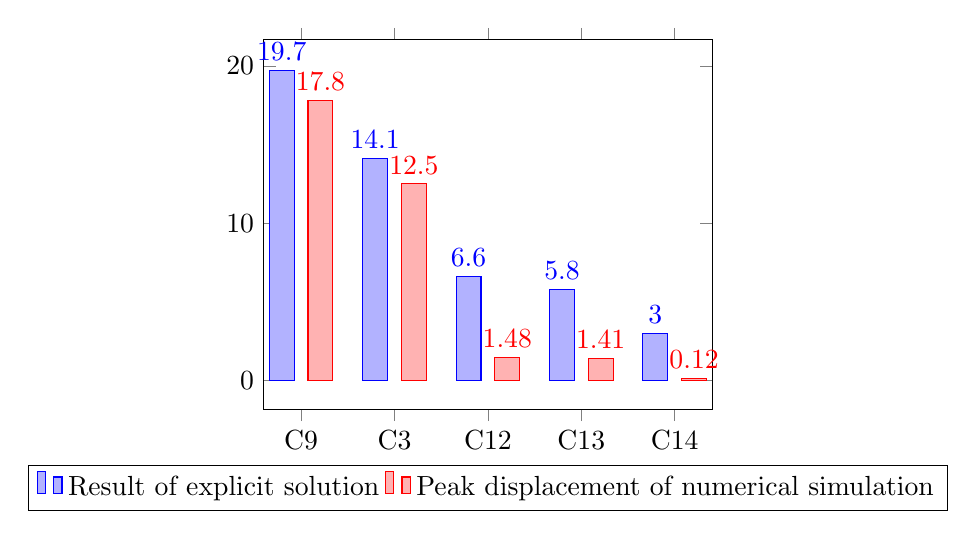
\begin{tikzpicture}
\begin{axis}[
	width = 0.6\textwidth,
    symbolic x coords={C9,C3,C12,C13,C14},
    xtick=data,
    legend style={at={(0.5,-0.15)},
        anchor=north,legend columns=-1},
    ybar=5pt,% configures `bar shift'
    bar width=9pt,
    nodes near coords,
]
\addplot 
    coordinates {(C9, 19.7) (C3, 14.1)   (C12,6.6) (C13,5.8) 
        (C14, 3.0) };
\addplot 
    coordinates {(C9, 17.8) (C3, 12.5)  (C12,1.48) (C13,1.41)
         (C14,0.117) };
\legend{Result of explicit solution,Peak displacement of numerical simulation}
\end{axis}
\end{tikzpicture}
\caption{Comparison between VAMPIRE peak simulation result and analytical peak result}
\label{fig:comparisonpeaksimulationanalytical}
\end{figure}

\paragraph{Benchmark conclusion}

It can be seen that explicit solution results always keep a conservative margin above the numerical simulation results. 

Difference between explicit solution and numerical simulation result for C12,C13 and C14 is bigger compared to difference for C9 and C3. It is due to the fact that the amplitude $Q$ is calculated based on freight train lateral forces and freight trains induce greater lateral force compared to passenger trains and high speed trains(See Figure.\ref{fig:peaklateralforceregression}).

The descending trend of explicit solution results follows the descending trend of numerical simulation results perfectly regardless of train types. 

Thus considering above reasons, the model shows satisfying performance. However, since there are few data available as benchmark, this model is still not verified for real-life application.

\section{Supplementary parameter calculation and benchmark}\label{sec:supplementaryparametercalculation}
Although the hypothesis expression based on C1 has been validated, this process is not generic because C1 is chosen specifically. To be scientific it is also necessary to derive expression of amplitude $Q$ based on other 5 simulation cases. 

The load equivalent amplitude of other 5 setups are calculated and their constant component are presented in the Table.\ref{tab:allLoadEquivalentAmplitude}. Their corresponding benchmarks are presented in Table.\ref{tab:allBenchmark}. Calculation processes are omitted because they are conducted in the same way as C1-based amplitude $Q$.

\begin{table}[h!]
    \centering
    \caption{Constant component of amplitude $Q$($N$) from all available setups}
    \begin{tabular}{cccccc}
        \hline
        C1 & C3 & C9 & C12 & C13 & C14 \\
        \hline
        1928 & 1721 & 1760 & 427 & 463 & 228 \\
        \hline
    \end{tabular}
    \label{tab:allLoadEquivalentAmplitude}
\end{table}

\begin{table}[h!]
	\tiny
    \centering
    \caption{Benchmark of explicit solution results}
    \begin{tabularx}{\textwidth}{XXXXXXX}
        \hline
         & \multicolumn{6}{c}{Analytical results of cases}\\
        \cline{2-7}
        Base simulation cases for $Q$ & C1 & C3 & C9 & C12 & C13 & C14 \\
        \hline
        C1 & 0.0145 & 0.0141 & 0.0197 & 0.0066 & 0.0058 & 0.003 \\
        C3 & 0.013 & 0.0125 & 0.0174 & 0.0059 & 0.0051 & 0.0036 \\
        C9 & 0.013 & 0.0128 & 0.0178 & 0.0061 & 0.0053 & 0.0032 \\
        C12 & 0.0032 & 0.0031 & 0.0043 & 0.00148 & 0.0013 & 0.0008 \\
        C13 & 0.0035 & 0.0034 & 0.0047 & 0.0016 & 0.00141 & 0.0002 \\
        C14 & 0.0021 & 0.0020 & 0.0028 & 0.0010 & 0.0008 & 0.00012 \\
        \hline
        Simulation Peak Displacement & 0.014 & 0.0125 & 0.0178 & 0.00148 & 0.00141 & 0.00012 \\
        \hline
        \label{tab:allBenchmark}
    \end{tabularx}
\end{table}

Among all amplitude $Q$, the one created from C1 is most satisfying because its outputs are all conservative towards numerical simulation output. Other  amplitude shows at least one nonconservative output. 

It can also be observed that the results of C12,C13 and C14 are unacceptable due to the reason that their output are too small compared to numerical simulation output . They can't predict reliable result for C1,C3 and C9.

Since there is few data available, it's meaningless to conduct further statistical procedures. The rest of the thesis will use amplitude $Q$ base C1 because it is conservative on all benchmark. 

\section{Evaluation on the model}
A simplified model for checking lateral resonance response of railway bridge is developed in this chapter. This model is capable of simulating a resonance scenario where the bridge is passed by a moving railway vehicle. However, several disadvantages of the current model should be noted:

\begin{enumerate}
	\item Only one concentrated force is modeled to represent the lateral dynamic effect induced by railway vehicle. It means the load in the model can not represent the distribution of vehicle axle forces. 
	\item Amplitude $Q$ is calculated based on a specifically chosen numerical simulation case. However, the aim of the model is to generically simulate vehicle-bridge response behavior, and such specifically choosing may be against this principle of generic.  
	\item The model is not fully validated because of the small quantity of available simulation results for validation. These simulation scenarios can not represent generic real-life scenarios.
	\item The model is not calibrated for modern Dutch railway because model parameter $Q$ is based on data generated by old railway vehicles.\footnote{Simulations\citep{d181dt329} were conducted during 1990s using parameters extracted from real trains at the time. Compared to trains of 1990s, modern railway vehicles possess more sophisticated suspension systems designed to suppress the lateral motion of the vehicle thus they are expected to induce lower lateral forces to tracks.} 
\end{enumerate}